\onecolumn
\chapter{Auswertung}
\label{ch:auswertung}

\section*{Fehlerrechnung}
Für die statistische Auswertung von $n$ Messwerten $x_i$ werden folgende Größen definiert \cite{errorSkript25}:
\begin{align}
    \bar{x} &= \frac{1}{n} \sum_{i=1}^{n} x_i \vphantom{\sqrt{\sum_i^n}^2} && \text{\textcolor{gray}{Arithmetisches Mittel}} \label{eq:arithmetisches_mittel} \\
    \sigma^2 &= \frac{1}{n-1} \sum_{i=1}^{n} (x_i - \bar{x})^2 \vphantom{\sqrt{\sum_i^n}^2} && \text{\textcolor{gray}{Variation}} \label{eq:variation} \\
    \sigma &= \sqrt{\frac{1}{n-1} \sum_{i=1}^{n} (x_i - \bar{x})^2} \vphantom{\sqrt{\sum_i^n}^2} && \text{\textcolor{gray}{Standardabweichung}} \label{eq:standardabweichung} \\
    \Delta \bar{x} &= \frac{\sigma}{\sqrt{n}} = \sqrt{\frac{1}{n(n-1)} \sum_{i=1}^n(\bar x - x_i)^2} \vphantom{\sqrt{\sum_i^n}^2} && \text{\textcolor{gray}{Fehler des Mittelwerts}} \label{eq:fehler_mittelwert} \\
    \Delta f &= \sqrt{\left(\frac{\partial f}{\partial x} \Delta x\right)^2 + \left(\frac{\partial f}{\partial y} \Delta y\right)^2} \vphantom{\sqrt{\sum_i^n}^2} && \text{\textcolor{gray}{Gauß’sches Fehlerfortpflanzungsgesetz für $f(x,y)$}} \label{eq:gauss_fehlfortpflanzung} \\
    \Delta f &= \sqrt{(\Delta x)^2 + (\Delta y)^2} \vphantom{\sqrt{\sum_i^n}^2} && \text{\textcolor{gray}{Fehler für $f = x + y$}} \label{eq:fehler_summe} \\
    \Delta f &= |a| \Delta x \vphantom{\sqrt{\sum_i^n}^2} && \text{\textcolor{gray}{Fehler für $f = ax$}} \label{eq:fehler_proportional} \\
    \frac{\Delta f}{|f|} &= \sqrt{\left(\frac{\Delta x}{x}\right)^2 + \left(\frac{\Delta y}{y}\right)^2} \vphantom{\sqrt{\sum_i^n}^2} && \text{\textcolor{gray}{relativer Fehler für $f = xy$ oder $f = x/y$}} \label{eq:relativer_fehler} \\
    \sigma &= \frac{|a_{lit} - a_{gem}|}{\sqrt{\Delta a_{lit}^2 + \Delta a_{gem}^2}} \vphantom{\sqrt{\sum_i^n}^2} && \text{\textcolor{gray}{Berechnung der signifikanten Abweichung}} \label{eq:signifikante_abweichung}
\end{align}

\twocolumn

%  ///////////////// AUFGABE 1 /////////////////
\section{Aufgabe 1: Pendellänge, Kugelradius und grobe Erdbeschleunigung}
\subsubsection*{Pendellänge}
Das Pendel wurde im Equilibrium vermessen. Es werden zwei Punkte an der Spiegelskala abgelesen, der obere un der untere Punkt der Kugel. Darüber hinaus wurde die Kugel mit der Schieblehre vermessen. So lässt sich die Fadenlänge und der Kugelradius jeweils auf zwei weisen Messen; jenachdem, welcher Messmethode man mehr vertrauen schencken mag.
Genutzt für die Messung wurden einmal die Spiegelskala, diese hat eine Skalapräzission von $0,10cm$, und einen geschätzten Ablesefehler von $0,3cm$, dieser Wert wurde großzügiger angenommen, da durch die Pendelbewegung das menschliche Auge Probleme beim Ablesen hat. Der wird aber für statische Rechnungen auf die Hälfte der Präzission angenommen. Ein systematischer Fehler ist hier nicht vermerkt. Die Gesamtungenauigkeit der Spiegelskala $\Delta s_{ss}$ wird via \hyperref[eq:gauss_fehlfortpflanzung]{Gauß'scher Fehlerfortpflanzung (\ref*{eq:gauss_fehlfortpflanzung})} bestimmt:
\begin{equation}
    \Delta s_{ss} = \sqrt{0,1^2+0,05^2} = 0,1118 \,[cm].
\end{equation}

Die Ungenauigkeit wurde hier auf signifikante Stellen gerundet.

Die Ungenauigkeit der Schieblehre lässt sich Analog bestimmen. Wir haben eine Präzission von $0,1cm$, aus welcher wir den Ableseungenauigkeit bestimmen, indem wir den Wert zu $0,05cm$ halbieren. Zuletzt gibt der Hersteller eine systematische Ungenauigkeit von $0,005cm$ an. Über die \hyperref[eq:gauss_fehlfortpflanzung]{Gauß'scher Fehlerfortpflanzung (\ref*{eq:gauss_fehlfortpflanzung})} berechnet sich der Gesamtfehler der Schieblehre:
\begin{equation}
    \Delta s_{sl} = \sqrt{0,1^2+0,05^2+0,005^2} = 0,1119 \, [cm].
\end{equation}
Auch dieses Ergebnis ist auf signifikante Stellen gerundet. Im statischen Zustand sind die beidne Methoden also annährend gleichgenau.

Der Durchmesser der Kugel ist gemessen mit der Schieblehre:
\begin{equation}
    \boxed{
        D_{k,sl} = (3,0000 \pm 0,1118)cm.
    }
\end{equation}

Man kann den Durchmesser jedoch auch über den die Diffrenz der beiden Fadenlängen bemessen. Wir haben hier drei Messwerte, daher nehmen wir den Mittelwert als Durchmesser der Kugel. Die Gemessenen Werte sin der Tabelle 1 des \hyperref[Protokoll]{Protokolls} zu entnehmen. Die Länge des Fadens ist dabei das \hyperref[eq:arithmetisches_mittel]{arithmetische Mittel \ref*{eq:arithmetisches_mittel}}. Wir entnehmen der Tabelle wieder die Werte und kommen auf eine Fadenlänge $l'$ von
\begin{equation}
    \boxed{
        l' = (88,1667 \pm 0,1119) cm.
    }
\end{equation}

Das Pendel ist hier definiert als die Fadenlänge und dem Radius der Kugel, da dort der Schwerpunkt der Kugel liegt. Die Fadenlänge inklusive des Durchmessers der Kugel $l_D$ ist das arithmetische Mittel der unteren Punkte:
\begin{equation}
    \boxed{
        l_D = (91,2000 \pm 0,118) cm.
    }
\end{equation}

Aus diesen Beiden Werten können die den Durchmesser der Kugel erneut bestimmenl, indem wir die Differenzen nehmen und kommen somit auf den Durchmesser
\begin{equation}
    \boxed{
        D_{k,ss} = (3,17 \pm 0,16)cm.
    }
\end{equation}

Der Fehler wurde über die \hyperref[eq:gauss_fehlfortpflanzung]{Gauß'scher Fehlerfortpflanzung (\ref*{eq:gauss_fehlfortpflanzung})} bestimmt, denn hier wurde die Differenz zwei fehlerbehafteten Werte gezogen:
\begin{equation}
    \Delta D_{k,ss} = \sqrt{2 \cdot 0,1118^2} = 0,16 \, [cm]
\end{equation}

Die Radien sind sehr ähnlich, jedoch haben sie eine recht große Abweichung. Berechnen wir die signifikante Abweichung der beiden Radien nach \hyperref[eq:signifikante_abweichung]{Gleichung \ref*{eq:signifikante_abweichung}}:
\begin{equation}
    \frac{\left| D_{k,ss} - D_{k,sl} \right|}{\sqrt{(\Delta s_{ss})^2 + (\Delta s_{sl})^2 }} = 0,85\sigma.
\end{equation}

Wir sehen, dass die Werte sich grundlegend Decken, jedoch spürbare unterschiede haben. Wir wollen das Ergebnis in der \hyperref[ch:diskussion]{Diskussion} diskutieren. Wir werden mit dem Bestimmten Radius der Schieblehre weiter rechnen, da der Wert >>satischer<< ist und sich hier weniger Bewegungsungenauigkeiten vermuten lassen.

Unser Kugelradius ist somit 
\begin{equation}
    \boxed{
        r_K = (1,50 \pm 0,06)cm.
    }
\end{equation}

Das Pendel hat somit eine Länge $l$ der Summe der Fadenlänge und des Kugelradiuses. Der der Pendellänge ist dabei:
\begin{equation}
    \Delta l = \sqrt{(\Delta r_K)^2 + (\Delta s_{ss})^2} = 0,13 \, [cm].
\end{equation} 

Das Pendel hat also eine Länge von
\begin{equation}
\boxed{
    l = (89,67 \pm 0,13)cm
}
\end{equation}


%  ///////////////// AUFGABE 2 /////////////////
\subsection*{Grobe Bestimmung der Erdbeschleunigung}
Im Aufgabenteil 2 wird eine Zeitgemessen. Wir wollen zunächst die Ungenauigkeit der Stoppuhr $\Delta t_{su}$ besimme. Wir haben eine Präzission von $0,01s$, sein Ablese Fehler wird auf 50\% der Präzission geschätzt und liegt somit bei $0,005s$. Die Ungenauigkeit der Stoppuhr ist somit nach der \hyperref[eq:gauss_fehlfortpflanzung]{Gauß'scher Fehlerfortpflanzung (\ref*{eq:gauss_fehlfortpflanzung})}:
\begin{equation}
    \Delta t_{su} = \sqrt{(0,010^2 + 0,0005^2)} = 0,01118 \, [s]
\end{equation}

Da wir mehrere Einzelmessungen haben, müssen wir den \hyperref[eq:fehler_mittelwert]{Fehler des Mittelwerts (\ref*{eq:fehler_mittelwert})} berechnen. Dies ist dann die statistische Ungenauigkeit:
\begin{equation}
    \overline{\delta t} = 0,0019 \, [s]
\end{equation}

Zusätzlich wollen wir eine durchschnittliche menschliche Reaktionszeit von $\Delta t_{reak} 0,250s$ annehmen. Der gesamte Zeitfehler einer Zeitmessung liegt somit bei:
\begin{equation}
    \Delta t = \sqrt{(\Delta t_{su})^2+ (\Delta t_{reak})^2 + (\overline{\delta t})^2}
    \label{eq:f_zeit}
\end{equation}

Setzen wir alles ein, so ist unser Fehler somit
\begin{equation}
    \Delta t = 0,25 s.
\end{equation}

Wie zu erwarten dominiert die Reaktionszeit hier.

Wir wollen die durchschnittliche Periodendauer aus 5 Messungen bestimmen. Die Messwerte sin der Tabelle 2 des \hyperref[Protokoll]{Protokolls} zu entnehmen. Es wurden für jede Messung die Zeit für 20 Schwingung bestimmt, dadurch wird der Zeitfehler minimiert. Dividiert man die gemessene Zeit mit $20$, so kommen wir auf 5 Perioden dauern. Es wird wieder das \hyperref[eq:arithmetisches_mittel]{arithmetische mittel (\ref*{eq:arithmetisches_mittel})} gebildet. Alle Messwerte haben denselben Fehler $\Delta t$, dieser wird für die Ungenauigkeit der Periodendauer auch mit 20 dividiert. Das Ergebnis ist somit:
\begin{equation}
    \boxed{
        \Bar{T_0} = (1,8917 \pm 0,0125)s
    }
\end{equation}

Mit diesem Wert haben wir alles, was wir nach \hyperref[eq:g_ideal]{Gleichung \ref*{eq:g_ideal}} brauchen, um die Erdbeschleunigung $g$ zubestimmen. Die Ungenauigkeit wird via \hyperref[eq:fehler_g]{Gleichung \ref*{eq:fehler_g}} berechnet.
Für $g$ kommen wir auf ein (nicht signifikant gerundetes) Ergebnis von:
\begin{equation}
    \underline{
        g = 9,8924 \frac{m}{s^2}
    }.
\end{equation}

Die Ungenauigkeit berechnet sich zu
\begin{equation}
    \underline{
        \Delta g = 0,13
    }
\end{equation}


Es wird zusammengefasst und aufsignifikante Stellen gerundet:
\begin{equation}
\boxed{
    g  = ( 9,89 \pm 0,13) \frac{m}{s^2}
}.
\end{equation}

Es wird nun die \hyperref[eq:signifikante_abweichung]{signifikante Abweichung (\ref*{eq:signifikante_abweichung})} mit Literaturwert der Erdbeschleunigung für Heidelberg von $g_{lit} = 9,80984 \pm 2 \cdot 10{-5} m/s^2$ berechnet:
\begin{equation}
    \frac{\left| g_{lit} - g \right|}{\sqrt{(\Delta g)^2 + (\Delta g_{lit})^2}} = 0,62\sigma.
\end{equation}

Das Ergebnis ist also schon statistisch signifikant und bestätigt die heidelberger Ortskonstante $g_{lit}$. 

Wir wollen nun jedoch vor allem schauen, ob wir diesen Wert noch weiter präzisieren können, indem wir genauere Messungen unternehmen.


%  ///////////////// AUFGABE 3 /////////////////
\subsection*{Bestimmung der Erdbeschleunigung über 200 Schwinungen}

Nach \hyperref[eq:bedingung_n]{Gleichung \ref*{eq:bedingung_n}} hätten wir 1318 Schwinungen machen müssen. Dies wäre jedoch kaum bewerkstelligbar gewesen, welshalb wir nach Absprache 200 Perioden gemacht haben. Der Tabelle 3 des \hyperref[Protokoll]{Protokolls} ist die Messzeit zu entnehmen. Diese beträgt:
\begin{equation}
    t_{200} = (378,73 \pm 0,25)s,
\end{equation}

woraus wir direkt die Periodendauer bestimmen können:
\begin{equation}
    \underline{
        T_{200} = (1,89365 \pm 0,00125)s.
    }
\end{equation}

Wir bestimmen also nochmal die Erdbeschleunigung und kommen somit nach \hyperref[eq:g_ideal]{Geleichung \ref*{eq:g_ideal}} und \hyperref[eq:fehler_g]{Geleichung \ref*{eq:fehler_g}} zu einem Ergebnis von
\begin{equation}
    \boxed{
        g_{200} = (9,812 \pm 0,019)
    }.
\end{equation}

Wir schauen, ob dieser Wert genauer am literatur Wert $g_{lit}$ von Heidelberg liegt:
\begin{equation}
    \frac{\left| g_{lit} - g_{200} \right|}{\sqrt{(\Delta g_{200})^2 + (\Delta g_{lit})^2}} = 0,11\sigma.
\end{equation}

Das Ergbenis ist somit weitaus genauer als das, mit fünf Messwerten.

%  ///////////////// AUFGABE 4 /////////////////
\section{Aufgabe 2: Berechnung der Korrekturstherme}
Wir wollen jedoch noch genauere Ergebnisse bekommen und werden daher weitere Eigenschaften untersuchen. Zunächst nehmen wir \hyperref[eq:T_gesamt]{Gleichung \ref*{eq:T_gesamt}} und stellen sie nach $g$ (unserer Ortskonstanten) um:
\begin{equation}
    g = \frac{4\pi^2 l}{T^2} \left(1 + \frac{2r^2}{5l^2} + \frac{\rho_L}{\rho_K} - \frac{m_F}{6 m_K} + \frac{\delta^2}{\omega_0^2} + \frac{\varphi_0^2}{8}\right).
    \label{eq:g_final}
\end{equation}

Damit lässt sich schön einsehen, welche Werte alles gebraucht werden. Dazu wollen wir erstmal die Therme berücksichtigen, die auf Materialeigenschaften basieren und zum anderen die Dämpfung. 

\subsection{Fehler durch Materialeigenschaften}
In der \hyperref[eq:g_final]{Gleichung \ref*{eq:g_final}} stehen verscheiedene Therme, die aus Materialgegebenheiten folgen. Wir haben dabei die Dichte der Luft $\rho_L$, die Dichte der Kugel $\rho_K$ und die daraus folgende Masse $m_K$. Außerdem brauchen wir die Masse des Fadens $m_l$. Für die dichten werden die Literaturwerte benutzt und als >>ideal<< angenommen. Das Material der Kugel ist mit Eisen angegeben.
\begin{align}
    \underline{\rho_L = 1,2 \cdot 10^{-3} \frac{g}{cm^3}} \\
    \underline{\rho_K = 7,86 \frac{g}{cm^3}}.
\end{align}

Für die Masse der Kugel müssen wir Ihr Volumen bestimmen. Für eine ideale Kugel gilt:
\begin{equation}
    V_K = \frac{4}{3} \cdot \pi \cdot {r_K}^3,
\end{equation}
mit einer Ungenauigkeit von
\begin{equation}
    \Delta V_K = 4 \cdot \pi \cdot {r_K}^2 \cdot \Delta r_K,
\end{equation}

Somit hat unsere Kugel ein Volumen von
\begin{equation}
    \underline{
        V_K = (14,1 \pm 1,7) cm^3.
    }
\end{equation}

Damit können wir die Masse zu 
\begin{equation}
    \boxed{
        m_k = (111 \pm 13) g.
    }
\end{equation}

Wir müssen zudem die Fadenmasse $m_f$ bestimmen. Die Fadenlänge $l'$ wurde bereits bestimmt. Wir nehmen für die Fadendichte dieselebe wie für die Kugel $\rho_f = \rho_K$. Der Radius ist im Skript mir $r_f = 0,01cm$ angegeben \cite{skript25}.
Die Masse des Fadens berechnet sich via
\begin{equation}
    m_f = \pi \cdot {r_f}^2 \cdot l' \cdot \rho_f,
\end{equation}

mit einer Ungenauigkeit von
\begin{equation}
    \Delta m_f = \pi \cdot {r_f}^2 \cdot \rho_f \cdot \Delta l'.
\end{equation}

Wir setzen besagte Werte ein und kommen auf eine Fadenmasse von
\begin{equation}
    \boxed{
        m_f = (0,21771 \pm 0,00028) \, g.
    }
\end{equation}

\subsection{Fehler durch Dämpfung}
Nun soll die Werte für $\varphi_0$ und für $\delta$ aus \hyperref[eq:g_final]{Gleichung \ref*{eq:g_final}}. Die Bestimmung von $\delta$ erfolgt graphisch, via der Werte aus Aufgabe 4 des \hyperref[Protokoll]{Protokolls}. 
Das Equilibrium des Pendles ist auf der horizontalen Skala bei 12cm. Die in der Tabelle eingetragenen Amplituden sind nicht die Auslenkungen, sondern der tatsächliche Skalenwert. Über die differenz des Equilibriums und der Auslenkung, bekommen wir die (ungefähre) Auslenkung.
Die benutze Spiegelskala hat eine Präzission von $0,1cm$, wir haben den Fehler jedoch höher geschätzt, da durch die Bewegung ein genaues Ablesen kaum möglich ist. Der Graph ist auf semilogarithmischen Papier gezeichnet.
Die Ungenauigkeit der Zeit wurde auf die Reaktionszeit des Menschen von circa $\Delta s_{reak} = 0,3s$ geschätzt und ist somit zu klein, um diese sinnvoll einzuzeichnen. Der Plot ist in \hyperref[fig:plot]{Abbildung \ref*{fig:plot}} zu finden.

Es handelt sich um eine exponentielle Abnahme. Die allgemeine Geleichung ist:
\begin{equation}
    a(t) = a_0 \cdot e^{-\delta t}
\end{equation}
Diese Gleichung soll nach $delta$ aufgelöst werden. Hierzu wird der deaktische Logartithmus ($\lg$) genutzt:
\begin{align}
    \lg(a(t)) &= \lg(a_0) + \lg(e^{-\delta t}) \\ 
    \notag &\Longleftrightarrow \\
    \delta &= \frac{\lg(a_0) - \lg (a(t))}{\lg(e) \cdot t}.
\end{align}

Nun wird $\delta$ für die Ausgleichsgerade (blau) und die Fehlergerade (orange) bestimmt.
\begin{align}
    \delta_A &= \frac{\lg(7,1) - \lg(3,4)}{\lg(e) \cdot 325,6s} = \underline{0,001920 s^{-1}}\\
    \delta_F &= \frac{\lg(7,3) - \lg(4,4)}{\lg(e) \cdot 360,92s} = \underline{0,0014027 s^{-1}}
\end{align}

Die finale Dämpfung ergibt sich somit zu 
\begin{equation}
\boxed{
    \delta = (1,9 \pm 0,5) \cdot 10^{-3} s^{-1}
}.
\end{equation}

Weitergehend geht es um die Berechnung von $\varphi_0$. Zur Berechnung dieses Winkels wird die Pendellänge $l$, sowie die mittlere Auslenkung genutzt. Porblematisch ist hier, dass bei Ablesen der Skala das obere Ende der Kugel und nicht der Mittelpunkt genutzt wurde. Jedoch wird dies mitunter durch den großen Ablesefehler von $\Delta = 0,3cm$ kompensiert. Die mittlere Auslenkung berechnet sich über das \hyperref[eq:arithmetisches_mittel]{Arithmetische Mittel (\ref*{eq:arithmetisches_mittel})}:
\begin{equation}
    \underline{
        \overline{A} = (4,59 \pm 0,30) cm.
    }
\end{equation}

Die Ungenauigkeit ist dabei der \hyperref[eq:fehler_mittelwert]{Fehler des Mittelwerts (\ref*{eq:fehler_mittelwert})}.

Über den Zusammenhang
\begin{equation}
\sin \varphi_0 = \frac{\bar x}{l}
\end{equation}
können wir den Winkel zu
\begin{equation}
    \varphi_0 = \arcsin \frac{\bar x}{l} 
\end{equation}
bestimmen. 
Über die \hyperref[eq:gauss_fehlfortpflanzung]{Gauß'sche Fehlerfortpflanzung (\ref*{eq:gauss_fehlfortpflanzung})} lässt sich zudem die Ungenauigkeit berechnen:
\begin{equation}
    \Delta \varphi_0 = \frac{1}{\sqrt{1 - (\bar x/l)^2}} \sqrt{{\left(\frac{\Delta \bar x}{\bar x}\right)^2 + \left(\frac{\bar x\Delta l}{l^2}\right)^2}}.
\end{equation}

Der berechnete Winkel liegt somit bei
\begin{equation}
    \boxed{
        \varphi_0 = (0,051 \pm 0,003) rad
    }.
\end{equation}

\onecolumn
\begin{figure}
    \hspace*{-2.4cm}
    \centering
    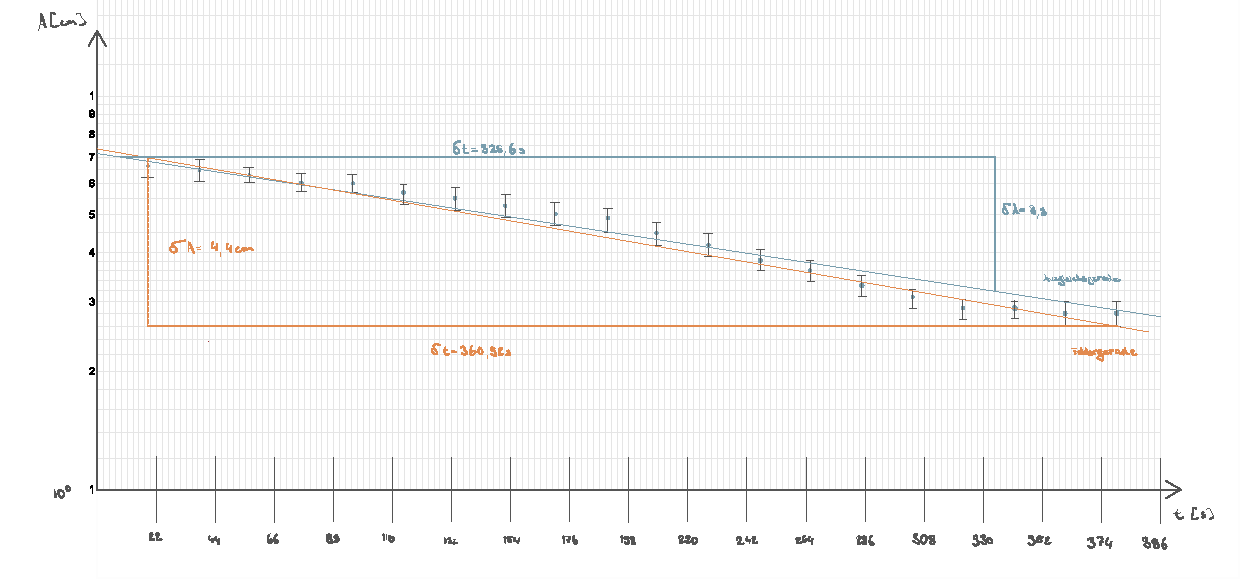
\includegraphics[width=1.3\textwidth]{img/14/BetterPlot.pdf}
    \caption{Amplitudenasulenkung des Pendels gegen die Zeit. Bleu ist die Ausgleichsgerade und orange die Fehler gerade. $\delta$ bedeutet hier die Differenz. Dies ist nicht dasselbe Delta, das gesucht ist.}
    \label{fig:plot} 
\end{figure}
\twocolumn

\subsection{Berechnung mit Korrektursthermen}
Nun sind alle Therme für \hyperref[eq:g_final]{Gleichung \ref*{eq:g_final}} bestimmt. Den Fehler für $g$ bestimmen wir überr die \hyperref[eq:gauss_fehlfortpflanzung]{Gauß'sche Fehlerfortpflanzung (\ref*{eq:gauss_fehlfortpflanzung})}:
\begin{align*}
    \Delta g = \Bigg[
    &\left( \left(\frac{g}{l} - \frac{16\pi^2 r^2}{5T^2 l^2}\right)\Delta l \right)^2
    + \left( \frac{2g}{T}\Delta T \right)^2 \\
    &+ \left( \frac{16\pi^2 r}{5T^2 l}\Delta r \right)^2
    + \left( \frac{4\pi^2 l}{6T^2 m_K}\Delta m_F \right)^2 \\
    &+ \left( \frac{4\pi^2 l m_F}{6T^2 m_K^2}\Delta m_K \right)^2
    + \left( \frac{8\pi^2 l\delta}{T^2 \omega_0^2}\Delta\delta \right)^2 \\
    &+ \left( \frac{8\pi^2 l\delta^2}{T^2 \omega_0^3}\Delta\omega_0 \right)^2
    + \left( \frac{\pi^2 l\varphi_0}{T^2}\Delta\varphi_0 \right)^2
    \Bigg]^{1/2}.
\end{align*}

Wir setzen alle unsere berechneten Werte in die Gleichungen ein und kommen auf ein korrigiertes Ergebnis:
\begin{equation}
    \boxed{
        g_K = (9,809 \pm 0,019) \frac{m}{s^2}
    }
\end{equation}

Für diese Rechnung wurde die durchschnittliche Periode erneut über die Werte aus Aufgabe 4 bestimmt und der Fehler über die \hyperref[eq:fehler_mittelwert]{Ungenauigkeit des Mittelwerts (\ref*{eq:fehler_mittelwert})}. Dieser Wert soll zunächst mit dem heidelberger Literaturwert verglichen werden (\ref{eq:signifikante_abweichung}):
\begin{equation}
    \frac{\left| g_K - g_{lit} \right|}{\sqrt{(\Delta g_K)^2 + (\Delta g_{lit})^2}} = 0,04\sigma.
\end{equation}

Dieser Wert soll auch mit dem $g_{200}$-Wert verglichen werden:
\begin{equation}
\frac{\left| g_{200} - g_K \right|}{\sqrt{(\delta g_{200})^2 + (\Delta g_K)^2}} = 0,11 \sigma
\end{equation}

